\documentclass[11pt]{article}
\usepackage{deauthor,times,graphicx}
\usepackage{amssymb}

\usepackage{xkvltxp}
\usepackage{fixme}

\graphicspath{{authorname/}}

%
% Paper size: 6 to 15 pages, single column
% additional info: http://tab.computer.org/tcde/bull_author.html
% deadline: end of January 2016
%

\newcommand{\ex}{$\mathcal{E}$}
\newcommand{\pp}{$\mathcal{P}$}
\newcommand{\ppm}{\mathcal{P}}
\newcommand{\cc}{$\mathcal{C}$}
\newcommand{\ccm}{\mathcal{C}}
\newcommand{\vv}{$\mathcal{V}$}
\newcommand{\vvm}{\mathcal{V}}
\newcommand{\vvt}{$\mathcal{V}$}
\newcommand{\rr}{$\mathcal{R}$}
\newcommand{\rrm}{\mathcal{R}}
\newcommand{\sst}{$\mathcal{S}$}
\newcommand{\ssm}{\mathcal{S}}
%
% S-SMR
\newcommand{\ssmr}{\mbox{S-SMR}}
\newcommand{\ssmrshort}{Scalable SMR}
\newcommand{\ssmrlong}{Scalable State Machine Replication}
%
% DS-SRM
\newcommand{\dssmr}{\mbox{DS-SMR}}
\newcommand{\dssmrshort}{Dynamic S-SMR}
\newcommand{\dssmrlong}{Dynamic Scalable State Machine Replication}
%
% Eyrie and Chirper temporary name (double blind)
\newcommand{\libname}{Eyrie}    % rename to Eyrie   after paper is accepted
\newcommand{\appname}{Chirper} % rename to Chirper after paper is accepted
%
\newcommand{\rmcast}{reliable-multicast}
\newcommand{\rmdel}{reliable-deliver}
\newcommand{\amcast}{atomic-multicast}
\newcommand{\amdel}{atomic-deliver}

\begin{document}

\title{Strong Consistency at Scale}

\author{
  Carlos Eduardo Bezerra\\
  University of Lugano (USI)\\
  Switzerland
  \and
  Le Long Hoang\\
  University of Lugano (USI)\\
  Switzerland
  \and
  Fernando Pedone\\
  University of Lugano (USI)\\
  Switzerland
}

\maketitle

\begin{abstract}
Today's online services must meet strict availability and performance requirements.
State machine replication, one of the most fundamental approaches to increasing the availability of services without sacrificing strong consistency, provides configurable availability but limited performance scalability.
Scalable State Machine Replication (S-SMR) achieves scalable performance by partitioning the service state and coordinating the ordering and execution of commands.
While S-SMR scales the performance of single-partition commands with the number of deployed partitions, replica coordination needed by multi-partition commands introduces an overhead in the execution of multi-partition commands.
In the paper, we review Scalable State Machine Replication and quantify the overhead due to replica coordination in different scenarios.
In brief, we show that performance overhead is affected by the number of partitions involved in multi-partition commands and data locality.
\end{abstract}

\section{Introduction}

In order to meet strict availability and performance requirements, today's online services must be replicated.
Managing replication without giving up strong consistency, however, is a daunting task.
State machine replication, one of the most fundamental approaches to replication~\cite{Lam78,Sch90}, achieves strong consistency (i.e., linearizability) by regulating how client commands are propagated to and executed by the replicas: every non-faulty replica must receive and execute every command in the same order. Moreover, command execution must be deterministic. 

State machine replication yields configurable availability but limited scalability.
Since every replica added to the system must execute all requests, 
increasing the number of replicas results in bounded improvements in performance.
%throughput does not steadily increase with the number of replicas.
Scalable performance can be achieved with state partitioning (also known as \emph{sharding}).
The idea is to divide the state of a service in multiple partitions so that most commands access one partition only and are equally distributed among partitions. 
Unfortunately, most services cannot be ``perfectly partitioned", that is, the service state cannot be divided in a way that commands access one partition only.
As a consequence, partitioned systems must cope with multi-partition commands.
Scalable State Machine Replication (S-SMR)~\cite{bezerra2014ssmr} divides the service state and replicates each partition. 
S-SMR relies on an atomic multicast primitive to consistently order commands within and across partitions. 
Commands that access a single partition are multicast to the concerned partition and executed as in classical SMR;
commands that involve multiple partitions are multicast to and executed at all concerned partitions.

Atomic multicast ensures that commands are consistently ordered within and across partitions---in brief, no two replicas deliver the same commands in different orders.
However, simply ordering commands consistently is not enough to ensure strong consistency in Scalable State Machine Replication since the execution of commands can interleave in ways that violate strong consistency.
In order to avoid consistency violations, S-SMR implements execution atomicity. 
With execution atomicity, replicas coordinate the execution of multi-partition commands.
Although the execution of any two replicas in the same partition does not need coordination, a replica in one partition must coordinate its execution with a replica in every other partition involved in a multi-partition command.

Execution atomicity captures real-time dependencies between commands, typical of strong consistency criteria such as linearizability and strict serializability.
In both linearizability and strict serializability, if one operation precedes another in real time (i.e., the first operation finishes before the second operation starts), then this dependency must be reflected in the way the two operations are ordered and executed.
Respecting real-time dependencies leads to replicated systems that truly behave like single-copy systems, and thus are easier to program.
Serializability does not need execution atomicity but may lead to non-intuitive behavior.
We show in the paper that execution atomicity is not as expensive to implement in a partitioned system as one might expect.

S-SMR has proved to provide scalable performance, in some cases involving single-partition commands, with improvements in throughput that grow linearly with the number of partitions~\cite{bezerra2014ssmr}.
Forcing replicas in different partitions to coordinate to ensure strong consistency may slow down the execution of multi-partition commands, since each replica cannot execute at its own pace (i.e., a fast replica in a partition may need to wait for a slower replica in a different partition).
%
This paper reviews the Scalable State Machine Replication approach and takes a close look at replica coordination in the execution of multi-partition commands.
%We seek to understand to which extent coordination among replicas slows down the execution of replicas in S-SMR.
For multi-partition commands that require replicas in different partitions to exchange data as part of the execution of the command, execution atomicity does not affect performance.
For multi-partition commands that do not require data exchange, execution atomicity has an impact on performance that depends on the number of partitions involved in the command and on data locality.
The more partitions are involved in a multi-partition command, the less the overhead introduced by execution atomicity is, varying from 53\% of performance overhead with two partitions to 12\% of overhead with 16 partitions.\fxfatal[draft]{Check this}
Moreover, the overhead is slightly higher in workloads that experience locality when compared to settings that do not present data locality.

%2P
%wi/s		wo/s
%8024		17242
%overhead = (17242 - 8024) / 17242 = 
%16P
%wi/s		wo/s
%19708	22443
%overhead = (22443 - 19708) / 22443 = 

The remainder of the paper is structured as follows.
Section~\ref{sec:sysmodel} presents the system model and definitions.
Sections~\ref{sec:smr} and \ref{sec:scalablesmr} recall classical state machine replication and scalable state machine replication.
Section~\ref{sec:perfeval} describes our experimental evaluation.
Section~\ref{sec:rwork} reviews related work and Section~\ref{sec:final} concludes the paper.

%\clearpage
\section{System model and definitions}
\label{sec:sysmodel}

\subsection{Processes and communication}

We consider a distributed system consisting of an unbounded set of client processes $\ccm = \{c_1, c_2, ...\}$ and a bounded set of server processes (replicas) $\ssm = \{s_1, ..., s_n\}$.
Set $\ssm$ is divided into disjoint groups of servers $\ssm_1, ..., \ssm_k$.
Processes are either \emph{correct}, if they never fail, or \emph{faulty}, otherwise.
In either case, processes do not experience arbitrary behavior (i.e., no Byzantine failures).
Each server group $S_i$ contains at least $f + 1$ correct processes, where $f$ is the number of faulty processes.

Processes communicate by message passing, using either one-to-one or one-to-many communication.
The system is asynchronous: there is no bound on message delay or on relative process speed.
One-to-one communication uses primitives $send(p,m)$ and $receive(m)$, where $m$ is a message and $p$ is the process $m$ is addressed to.
If sender and receiver are correct, then every message sent is eventually received.
%
One-to-many communication relies on reliable multicast and atomic multicast,\footnote{Solving atomic multicast requires additional assumptions~\cite{CT96,FLP85}. In the following, we simply assume the existence of an atomic multicast oracle.}
defined in sections~\ref{sec:rmcast} and \ref{sec:amcast}, respectively.
%Atomic broadcast is a special case of atomic multicast in which there is a single group with all servers.


\subsection{Reliable multicast}
\label{sec:rmcast}

To reliably multicast a message $m$ to a set of groups $\gamma$, processes use primitive \rmcast$(\gamma, m)$.
Message $m$ is delivered at the destinations with \rmdel$(m)$.
Reliable multicast has the following properties:

\begin{itemize}

    \item[--] If a correct process \rmcast{}s $m$, then every correct process in $\gamma$ \rmdel{}s $m$ \emph{(validity)}.

    \item[--] If a correct process \rmdel{}s $m$, then every correct process in $\gamma$ \rmdel{}s $m$ \emph{(agreement)}.

    \item[--] For any message $m$, every process $p$ in $\gamma$ \rmdel{}s $m$ at most once, and only if some process has \rmcast{} $m$  to $\gamma$ previously \emph{(integrity)}.

\end{itemize}

\subsection{Atomic multicast}
\label{sec:amcast}

To atomically multicast a message $m$ to a set of groups $\gamma$, processes use primitive \amcast$(\gamma, m)$.
Message $m$ is delivered at the destinations with \amdel$(m)$.
Atomic multicast ensures the following properties:

\begin{itemize}

    \item[--] If a correct process \amcast{}s $m$, then every correct process in $\gamma$ \amdel{}s $m$ \emph{(validity)}.

    \item[--] If a process \amdel{}s $m$, then every correct process in $\gamma$ \amdel{}s $m$ \emph{(uniform agreement)}.

    \item[--] For any message $m$, every process $p$ in $\gamma$ \amdel{}s $m$ at most once, and only if some process has \amcast{} $m$ to $\gamma$ previously \emph{(integrity)}.

    \item[--] No two processes $p$ and $q$ in both $\gamma$ and $\gamma'$ \amdel\ $m$ and $m'$ in different orders; also, the delivery order is acyclic \emph{(atomic order)}.

\end{itemize}

Atomic broadcast is a special case of atomic multicast in which there is a single group of processes.


%\subsection{Consistency criterion}
%
%Our consistency criterion is linearizability.
%A system is \emph{linearizable} if there is a way to reorder the client commands in a sequence that (i)~respects the semantics of the commands, as defined in their sequential specifications, and (ii)~respects the real-time precedence of commands~\cite{Attiya04}.



\section{State machine replication}
\label{sec:smr}

State machine replication is a fundamental approach to implementing a fault-tolerant service by replicating servers and coordinating the execution of client commands against server replicas~\cite{Lam78, Sch90}.
The service is defined by a state machine, which consists of a set of \emph{state variables} $\vvm = \{v_1, ..., v_m\}$
%that encode the service's state
and a set of \emph{commands} that may read and modify state variables, and produce a response for the command.
Each command is implemented by a deterministic program.
% whose execution is atomic with respect to other commands.
%The set of variables read by $C$ and the set of variables updated by $C$ are denoted, respectively, by $readset(C)$ and $writeset(C)$.
%The set of all variables read and updated by $C$ is denoted by $var(C)$.
State machine replication can be implemented with atomic broadcast: commands are atomically broadcast to all servers, and all correct servers deliver and execute the same sequence of commands.

We consider implementations of state machine replication that ensure linearizability.
%
Linearizability is defined with respect to a sequential specification.
The \emph{sequential specification} of a service consists of a set of commands and a set of \emph{legal sequences of commands}, which define the behavior of the service when it is accessed sequentially.
In a legal sequence of commands, every response to the invocation of a command immediately follows its invocation, with no other invocation or response in between them.
For example, a sequence of operations for a read-write variable $v$ is legal if every read command returns the value of the most recent write command that precedes the read, if there is one, or the initial value, otherwise.
An execution \ex\ is linearizable if there is some permutation of the commands executed in \ex\ that respects (i)~the service's sequential specification and (ii)~the real-time precedence of commands.
Command $C_1$ precedes command $C_2$ in real-time if the response of $C_1$ occurs before the invocation of $C_2$.

In classical state machine replication, throughput does not scale with the number of replicas: each command must be ordered among replicas and executed and replied by every (non-faulty) replica.
Some simple optimizations to the traditional scheme can provide improved performance but not scalability.
For example, although update commands must be ordered and executed by every replica, only one replica can respond to the client, saving resources at the other replicas.
Commands that only read the state must be ordered with respect to other commands, but can be executed by a single replica, the replica that will respond to the client.

%This is a fundamental limitation: while some optimizations may increase throughput by adding servers, the improvements are limited since fundamentally, the technique does not scale.
%In the next section, we describe an extension to SMR that under certain workloads allows performance to grow proportionally to the number of replicas.


\section{Scalable State Machine Replication}
\label{sec:scalablesmr}

In this section, we describe an extension to SMR that under certain workloads allows performance to grow proportionally to the number of replicas~\cite{bezerra2014ssmr}.
We first recall  S-SMR and then discuss some of its performance optimizations.

\subsection{General idea}
\label{sec:generalidea}

S-SMR divides the application state $\vvm$ (i.e., state variables) into $k$ partitions $\ppm_1, ..., \ppm_k$, where for each $\ppm_i$, $\ppm_i \subseteq \vvm$.
Moreover, we require each variable $v$ in $\vvm$ to be assigned to at least one partition and define $part(v)$ as the partitions that hold $v$.
Each partition $\ppm_i$ is replicated by servers in group $\ssm_i$.
For brevity, we say that server $s$ belongs to $\ppm_i$ with the meaning that $s \in \ssm_i$, and say that client $c$ multicasts command $C$ to partition $\ppm_i$ meaning that $c$ multicasts $C$ to group $\ssm_i$.
% We also say that $\ppm_i$ does something meaning that servers in $\ssm_i$.
%We also often mention $\ppm_i$ meaning servers in $\ssm_i$.

To execute command $C$, the client multicasts $C$ to all partitions that hold a variable read or updated by $C$.
Consequently, the client must be able to determine the partitions that may be accessed by $C$.
Note that this assumption does not imply that the client must know all variables accessed by $C$, nor even the exact set of partitions.
If the client cannot determine a priori which partitions will be accessed by $C$, it must define a superset of these partitions, in the worst case assuming all partitions.
For performance, however, clients must strive to provide a close approximation to the command's actually accessed partitions.
We assume the existence of an oracle that tells the client which partitions should receive each command.

Upon delivering command $C$, if server $s$ does not contain all variables read by $C$, $s$ must communicate with servers in other partitions to execute $C$.
Essentially, $s$ must retrieve every variable $v$ read in $C$ from a server that stores $v$ (i.e., a server in a partition in $part(v)$).
Moreover, $s$ must retrieve a value of $v$ that is consistent with the order in which $C$ is executed, as we explain next.
%Operations that do not involve reading a variable from a remote partition are executed locally.

In more detail, let $op$ be an operation in the execution of command $C$.
We distinguish between three operation types: $read(v)$, an operation that reads the value of a state variable $v$, $write(v, val)$, an operation that updates $v$ with value $val$,
and an operation that performs a deterministic computation.

Server $s$ in partition $\ppm_i$ executes $op$ as follows.

\begin{itemize}

\item[i)] \underline{$op$ is a $read(v)$ operation.} \\
If $\ppm_i \in part(v)$, then $s$ retrieves the value of $v$ and sends it to every partition $\ppm_j$ that delivers $C$ and does not hold $v$. If $\ppm_i \not\in part(v)$, then $s$ waits for $v$ to be received from a server in a partition in $part(v)$.

\item[ii)] \underline{$op$ is a $write(v,val)$ operation.} \\
If $\ppm_i \in part(v)$, $s$ updates the value of $v$ with $val$; if $\ppm_i \not\in part(v)$, $s$ executes $op$, creating a local copy of $v$, which will be up-to-date at least until the end of $C$'s execution.

\item[iii)] \underline{$op$ is a computation operation.}\\
In this case, $s$ executes $op$.

\end{itemize}

It turns out that atomically ordering commands and following the procedure above is not enough to ensure linearizability~\cite{bezerra2014ssmr}.
Consider the execution depicted in Figure~\ref{fig:mcastnonlinssmr}~(a), where state variables $x$ and $y$ have initial value of $10$.
Command $C_x$ reads the value of $x$, $C_y$ reads the value of $y$, and $C_{xy}$ sets $x$ and $y$ to value 20.
Consequently, $C_x$ is multicast to partition $\ppm_x$, $C_y$ is multicast to $\ppm_y$, and $C_{xy}$ is multicast to both $\ppm_x$ and $\ppm_y$.
Servers in $\ppm_y$ deliver $C_y$ and then $C_{xy}$, while servers in $\ppm_x$ deliver $C_{xy}$ and then $C_x$, which is consistent with atomic order.
In this execution, the only possible legal permutation for the commands is $C_y$, $C_{xy}$, and $C_x$, which violates the real-time precedence of the commands, since $C_x$ precedes $C_y$ in real-time.

\begin{figure*}
\begin{minipage}[b]{1.0\linewidth} % A minipage that covers the whole width of the page
\centering
      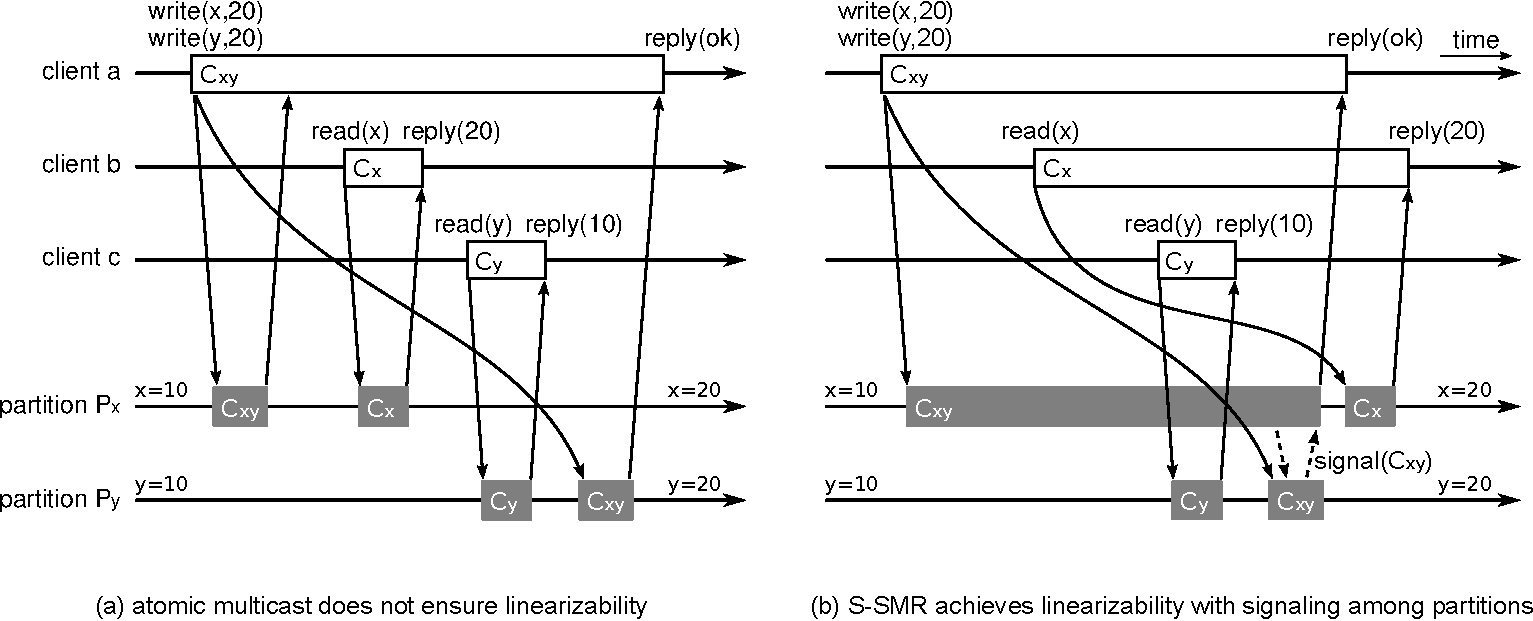
\includegraphics[width=0.85\linewidth]{mcastssmr_nonlin_linsignal_v3}
\end{minipage}
\caption{Atomic multicast and S-SMR. (To simplify the figure, we show a single replica per partition.)}
\label{fig:mcastnonlinssmr}
\end{figure*}

Intuitively, the problem with the execution in Figure~\ref{fig:mcastnonlinssmr}~(a) is that commands $C_x$ and $C_y$ execute ``in between'' the execution of $C_{xy}$ at partitions $\ppm_x$ and $\ppm_y$.
In S-SMR, we avoid such cases by ensuring that the execution of every command is atomic.
%
Command $C$ is \emph{execution atomic} if, for each server $s$ that executes $C$, there exists at least one server $r$ in every other partition in $part(C)$ such that the execution of $C$ at $s$ finishes only after $r$ starts executing $C$.
%
More precisely, let $start(C,p)$ and $end(C,p)$ be, respectively, the time when server $p$ starts executing command $C$ and the time when $p$ finishes $C$'s execution.
Execution atomicity ensures that, for every server $s$ in partition \pp\ that executes $C$, there is a server $r$ in every $\ppm' \in part(C)$ such that \mbox{$start(C,r) < end(C,s)$}.
Intuitively, this condition guarantees that the execution of $C$ at $s$ and $r$ overlap in time.

%Back in Fig.~\ref{fig:mcastnonlinssmr}, each black box represents the execution of a subcommand by servers in the partition: it starts when the first server in the partition begins executing the subcommand and ends when there is no more server executing the subcommand in that partition. We can see that $C_{xy}$ is not execution atomic: there is no time $t$ when some servers $s_x$ in $P_x$ and $s_y$ in $P_y$ are executing it. If it were the case, this example would be impossible to build, since $finish(C_y,s_y) < start(C_{xy}, s_y) < t < finish(C_{xy}, s_x) < start(C_x, s_x)$, which would contradict the fact that $C_x$ precedes $C_y$ in real-time.

Replicas can ensure execution atomicity by coordinating the execution of commands.
After starting the execution of command $C$, servers in each partition send a $signal(C)$ message to servers in the other partitions in $part(C)$.
Before finishing the execution of $C$ and sending a reply to the client that issued $C$, each server must receive a $signal(C)$ message from at least one server in every other partition that executes $C$.
Because of this scheme, each partition is required to have at least $f+1$ correct servers, where $f$ is the maximum number of tolerated failures per partition; if all servers in a partition fail, service progress is not guaranteed.

Figure \ref{fig:mcastnonlinssmr}~(b) shows an execution of S-SMR.
In the example, servers in $\ppm_x$ wait for a signal from $\ppm_y$,
therefore ensuring that the servers of both partitions are synchronized during the execution of $C_{xy}$.
Note that the outcome of each command execution is the same as in case (a), but the execution of $C_x$, $C_y$ and $C_{xy}$, as seen by clients, now overlap in time with one another.
Hence, there is no real-time precedence among them and linearizability is not violated.




\subsection{Performance optimizations}
\label{sec:optm}

The scheme described in the previous section can be optimized in many ways.
In this section, we briefly mention some of these optimizations and then detail caching.
\begin{itemize}
\item Server $s$ does not need to wait for the execution of command $C$ to reach a $read(v)$ operation to only then multicast $v$ to the other partitions in $part(C)$. If $s$ knows that $v$ will be read by $C$, $s$ can send $v$'s value to the other partitions as soon as $s$ starts executing $C$.
\item The exchange of objects between partitions serves the purpose of signaling. Therefore, if server $s$ sends variable $v$'s value to server $r$ in another partition, $r$ does not need to receive a signal message from $s$'s partition.
\item It is not necessary to exchange each variable more than once per command since any change during the execution of the command will be deterministic and thus any changes to the variable can be applied to the cached value.
\item Even though all replicas in all partitions in $part(C)$ execute $C$, a reply from a replica in a single partition suffices for the client to finish the command.
\end{itemize}

%Caching is a more elaborate optimization.
Server $s$ in partition \pp\ can cache variables that belong to other partitions.
There are different ways for $s$ to maintain cached variables; here we define two techniques: conservative caching and speculative caching.
In both cases, the basic operation is the following:
When $s$ executes a command that reads variable $x$ from some other partition $\ppm{}_x$, after retrieving the value of $x$ from a server in $\ppm{}_x$, $s$ stores $x$'s value in its cache and uses the cached value in future read operations.
If a command writes $x$, $s$ updates (or creates) $x$'s local value.
Server $s$ will have a valid cache of $x$ until (i)~$s$ discards the entry due to memory constraints, or (ii)~some command not multicast to \pp\ changes the value of $x$.
Since servers in $\ppm_x$ deliver all commands that access $x$, these servers know when any possible cached value of $x$ is stale.
How servers use cached entries distinguishes conservative from speculative caching.
%; what it does not know, however, is whether \pp\ has discarded $x$'s cache.


Servers in $\ppm_x$ can determine which of its variables have a stale value cached in other partitions. This can be done by checking if there was any command that updated a variable $x$ in $\ppm_x$, where such command was not multicast to some other partition $\ppm$ that had a cache of $x$. Say servers in $\ppm_x$ deliver command $C$, which reads $x$, and say the last command that updated the value of $x$ was $C_w$. Since $x \in \ppm_x$, servers in $\ppm_x$ delivered $C_w$. One way for servers in $\ppm_x$ to determine which partitions need to update their cache of $x$ is by checking which destinations of $C$ did not receive $C_w$. This can be further optimized: even if servers in $\ppm$ did not deliver $C_w$, but delivered some other command $C_r$ that reads $x$ and $C_r$ was ordered by multicast after $C_w$, then $\ppm$ already received an up-to-date value of $x$ (sent by servers in $\ppm_x$ during the execution of $C_r$). If servers in $\ppm$ discarded the cache of $x$ (e.g., due to limited memory), they will have to send a request for its value.


\emph{Conservative caching}: Once $s$ has a cached value of $x$, before it executes a $read(x)$ operation, it waits for a cache-validation message from a server in $\ppm_x$. The cache validation message contains a set of pairs $(var, val)$, where $var$ is a state variable that belongs to $\ppm_x$ and whose cache in $\ppm$ needs to be validated.
If servers in $\ppm_x$ determined that the cache is stale, $val$ contains the new value of $var$; otherwise, $\perp$, telling $s$ that its cached value is up to date.
If $s$ discarded its cached copy, it sends a request for $x$ to $\ppm_x$.
If it is possible to determine which variables are accessed by $C$ before $C$'s execution, all such messages can be sent upon delivery of the command, reducing waiting time; messages concerning variables that could not be determined a-priori are sent later, during the execution of $C$, as variables are determined.

\emph{Speculative caching}: It is possible to reduce execution time by speculatively assuming that cached values are up-to-date.
Speculative caching requires servers to be able to rollback the execution of commands, in case the speculative assumption fails to hold.
Many applications allow rolling back a command, such as databases, as long as no reply has been sent to the client for the command yet.
The difference between speculative caching and conservative caching is that in the former servers that keep cached values do not wait for a cache-validation message before reading a cached entry; instead, a $read(x)$ operation returns the cached value immediately.
If after reading some variable $x$ from the cache, during the execution of command $C$, server $s$ receives a message from a server in $\ppm_x$ that invalidates the cached value, $s$ rolls back the execution to some point before the $read(x)$ operation and resumes the command execution, now with the up-to-date value of $x$.
Server $s$ can only reply to the client that issued $C$ after every variable read from the cache has been validated.


\section{Performance evaluation}
\label{sec:perfeval}

In this section, we present the results found with \appname{}, a scalable social network application based on \ssmr{}.
We compare the performance impact of the \ssmr{} signaling mechanism, by running experiments with, and experiments without signaling turned on.
This was done for different workloads and numbers of partitions.
In Section~\ref{sec:evaluation:app}, we describe the implementation of \appname{}.
In Section~\ref{sec:evaluation:setup}, we describe the environment where we conducted our experiments.
In Section~\ref{sec:evaluation:result}, we report the results.

\subsection{\appname}
\label{sec:evaluation:app}

We implemented \appname{}, a social network application similar to Twitter, in order to evaluate the performance of \ssmr{}.
Twitter is an online social networking service in which users can post 140-character messages and read posted messages of other users.
The API of \appname{} includes: post (user publishes a message), follow (user starts following another user), unfollow (user stops following someone), and getTimeline (user requests messages of all people whom the user follows).

\appname{} partitions the state based on user id. A function $f(uid)$ returns the partition that contains all up-to-date information regarding user with id uid. Taking into account that a typical user probably spends more time reading messages (i.e., issuing getTimeline) than writing them (i.e., issuing post), we decided to optimize getTimeline to be single-partition. This means that, when a user requests his or her timeline, all messages should be available in the partition that stores that user's data, in the form of a materialized timeline (similarly to a materialized view in a database). To make this possible, whenever a post request is executed, the message is inserted into the materialized timeline of all users that follow the one that is posting. Also, when a user starts following another user, the messages of the followed user are inserted into the follower's materialized timeline as part of the command execution; likewise, they are removed when a user stops following another user. Because of this design decision, every getTimeline request accesses only one partition, follow and unfollow requests access objects on at most two partitions, and post requests access up to all partitions.

One detail about the post request is that it needs access to all users that follow the user issuing the post.
Since the \appname{} client cannot know for sure who follows the user, it keeps a cache of followers.
The client cache can become stale if a different user starts following the poster.
To ensure linearizability when executing a post request, the \appname\ server checks if the command is sent to the proper set of partitions. 
If this is the case, the request is executed.
Otherwise, the server sends a $retry(\gamma)$ message, where $\gamma$ is the complete set of additional partitions the command must be multicast to. Upon receiving the $retry(\gamma)$ message, the \appname\ client multicasts the command again, now with the destination that includes all partitions in $\gamma$. This repeats until all partitions that contain followers of the poster deliver the command. This is guaranteed to terminate because partitions are only added to the set of destinations for retries, never removed. Therefore, in the worst case scenario, the client will retry until it multicasts the post request to all partitions of the system.

Moreover, in order to observe the impact of the signaling mechanism described above, we also introduced these two commands: Follow-noop and Unfollow-noop, which demonstrate pure signal exchange, since they do not change the structure of the social network (i.e., do not change the list of followers and followed users).


\subsection{Environment setup and configuration parameters}
\label{sec:evaluation:setup}

All experiments were conducted on a cluster that had two types of nodes: (a) HP SE1102 nodes, equipped with two Intel Xeon L5420 processors running at 2.5 GHz and with 8 GB of main memory, and (b) Dell SC1435 nodes, equipped with two AMD Opteron 2212 processors running at 2.0 GHz and with 4 GB of main memory. The HP nodes were connected to an HP ProCurve 2920-48G gigabit network switch, and the Dell nodes were connected to another, identical switch. Those switches were interconnected by a 20 Gbps link.
All nodes ran CentOS Linux 7.1 with kernel 3.10 and had the OpenJDK Runtime Environment~8 with the \mbox{64-Bit} Server VM (build 25.45-b02).
We kept the clocks synchronized using NTP in order to measure latency components involving events in different computers.

For the experiments, we used the following workloads:
Timeline (composed only of getTimeline requests),
Post (only post requests), and
Follow/unfollow (50\% of follow-noop requests and 50\% of unfollow-noop).


\subsection{Results}
\label{sec:evaluation:result}

For the Timeline workload, the throughput and latency when signaling was turned on and off are very similar (see Figure~\ref{fig:perf}).
This happens because getTimeline requests are optimized to be single-partition:
all posts in a user's timeline are stored along with the User object.
Every getTimeline request accesses a single User object (of the user whose timeline is being requested).
The whole structure and content of the network do not change, and partitions do not need to exchange either signal or data.
Thus, enabling or disabling signal would not affect the performance of \appname{} when executing only getTimeline requests.

\begin{figure*}
\begin{minipage}[b]{1\linewidth} % A minipage that covers the whole width of the page
\centering
      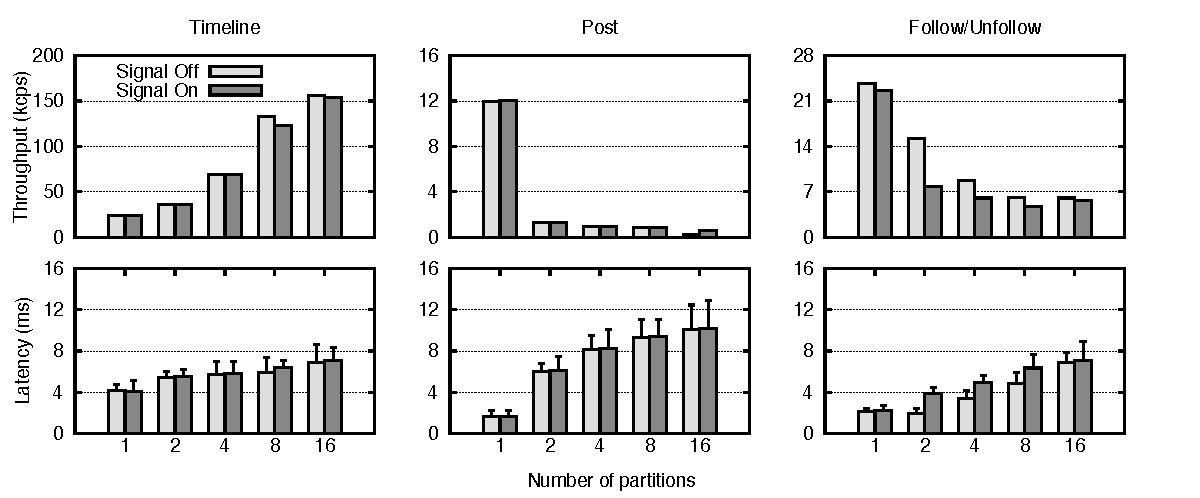
\includegraphics[width=1\linewidth]{figures/sc-at-scale-balance}
\end{minipage}
\caption{Results of \appname\ running with signaling turned on and off, on a balanced dataset. Throughput is shown in thousands of commands per second (kcps). Latency is measured in milliseconds (bars show average and whiskers show 95-th percentile).}
\label{fig:perf}
\end{figure*}

\begin{figure*}
\begin{minipage}[b]{1\linewidth} % A minipage that covers the whole width of the page
\centering
      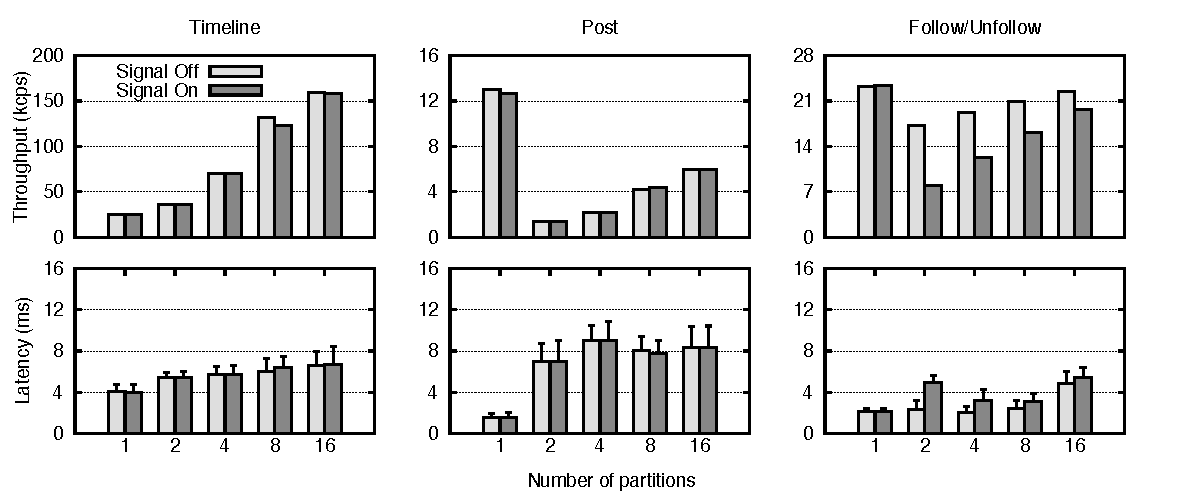
\includegraphics[width=1\linewidth]{figures/sc-at-scale-locality}
\end{minipage}
\caption{Results of \appname\ running with signaling turned on and off, on a dataset with locality. Throughput is shown in thousands of commands per second (kcps). Latency is measured in milliseconds (bars show average and whiskers show 95-th percentile).}
\label{fig:perf}
\end{figure*}


In the Post workload, every command accesses up to all partitions in the system, which requires partitions to exchange both data and signals.
In the execution with only one partition, where signals and data are not exchanged anyway, turning off signaling does not change performance.
With two partitions or more, signals and data are exchanged across partitions. 
However, we can see that the signaling does not affect the performance of \appname{} significantly. This happens because the Post command changes the content of the User object (changes in timeline), so in both tests, partitions have to exchange data anyhow. For this reason, even when signaling is turned off, the partitions still have to communicate. As a result, the throughput and delay with signaling turned on or off are similar.

In the Follow/unfollow workload, each command accesses up to two partitions in the system, requires partitions to exchange signal (no data exchanged since the noop command does not change the content of the network).
With one partition, \appname{} performs in a similar way to that observed with the Post workload in the experiment with one partition.
With two partitions or more, performance of \appname{} decreased when signaling was turned on. 
This was expected since the partitions started to exchange the signals: partitions had to wait for signal during the execution of the command.




\section{Related work}
\label{sec:rwork}

State machine replication is a well-known approach to replication and has been extensively studied (e.g., \cite{Lam78, Sch90, kapritsos2012eve, kotla2004htbft, santos2013htsmr}).
State machine replication requires replicas to execute commands deterministically, which implies sequential execution.
Even though increasing the performance of state machine replication is non-trivial, different techniques have been proposed for achieving scalable systems, such as optimizing the propagation and ordering of commands (i.e., the underlying atomic broadcast algorithm).
In \cite{kapritsos2010scalable}, the authors propose to have clients send their requests to multiple computer clusters, where each such cluster executes the ordering protocol only for the requests it received, and then forwards this partial order to every server replica.
The server replicas, then, must deterministically merge all different partial orders received from the ordering clusters.
In~\cite{biely2012spaxos}, Paxos~\cite{Lam98} is used to order commands, but it is implemented in a way such that the task of ordering messages is evenly distributed among replicas, as opposed to having a leader process that performs more work than the others and may eventually become a bottleneck.

State machine replication seems at first to prevent multi-threaded execution since it may lead to non-determinism.
However, some works have proposed multi-threaded implementations of state machine replication, circumventing the non-determinism caused by concurrency in some way.
In \cite{santos2013htsmr}, for instance, the authors propose organizing each replica in multiple modules that perform different tasks concurrently, such as receiving messages, batching, and dispatching commands to be executed.
The execution of commands is still sequential, but the replica performs all other tasks in parallel. 
%We also implemented this kind of parallelism in Eyrie.

Some works have proposed to parallelize the execution of commands in SMR.
In \cite{kotla2004htbft}, application semantics is used to determine which commands can be executed concurrently without reducing determinism (e.g., read-only commands can be executed in any order relative to one another).
Upon delivery, commands are directed to a parallelizer thread that uses application-supplied rules to schedule multi-threaded execution.
Another way of dealing with non-determinism is proposed in \cite{kapritsos2012eve}, where commands are speculatively executed concurrently.
After a batch of commands is executed, replicas verify whether they reached a consistent state; if not, commands are rolled back and re-executed sequentially.
Both \cite{kotla2004htbft} and \cite{kapritsos2012eve} assume a Byzantine failure model and in both cases, a single thread is responsible for receiving and scheduling commands to be executed.
In the Byzantine failure model, command execution typically includes signature handling, which can result in expensive commands.
Under benign failures, command execution is less expensive and the thread responsible for command reception and scheduling may become a performance bottleneck.
%For commands that take long to execute, this may not be a problem, but for workloads where the command execution time is shorter than the parallelization time, those approaches may not scale.

Many database replication schemes also aim at improving the system throughput, although commonly they do not ensure strong consistency as we define it here (i.e., as linearizability). Many works (e.g., \cite{chundi96dur, kobus2013hybrid, sciascia2012sdur, SousaOMP01}) are based on the deferred-update replication scheme, in which replicas commit read-only transactions immediately, not necessarily synchronizing with each other. This provides a significant improvement in performance, but allows non-linearizable executions to take place. The consistency criteria usually ensured by database systems are serializability \cite{BHG87} or snapshot isolation \cite{LinKJPA09}. Those criteria can be considered weaker than linearizability, in the sense that they do not take into account real-time precedence of different commands among different clients. For some applications, this kind of consistency is good enough, allowing the system to scale better, but services that require linearizability cannot be implemented with such techniques.

Other works have tried to make linearizable systems scalable~\cite{corbett2013spanner, Glendenning2011, Marandi11}.
In \cite{Glendenning2011}, the authors propose a scalable key-value store based on DHTs, ensuring linearizability, but only for requests that access the same key.
In \cite{Marandi11}, a partitioned variant of SMR is proposed, supporting single-partition updates and multi-partition read operations.
It relies on total order: all commands have to be ordered by a single sequencer (e.g., a Paxos group of acceptors), so that linearizability is ensured.
The replication scheme proposed in \cite{Marandi11} does not allow multi-partition update commands.
Spanner~\cite{corbett2013spanner} uses a separate Paxos group per partition.
To ensure strong consistency across partitions, it assumes that clocks are synchronized within a certain bound that may change over time.
The authors say that Spanner works well with GPS and atomic clocks.

Scalable State Machine Replication employs state partitioning and ensures linearizability for any possible execution, while allowing throughput to scale as partitions are added, even in the presence of multi-partition commands and unsynchronized clocks.

\section{Final remarks}
\label{sec:final}

This paper described S-SMR, a scalable variant of the well-known state machine replication technique.
S-SMR differs from previous related works in that it allows throughput to scale with the number of partitions without weakening consistency.
We evaluate S-SMR with Chirper, a scalable social network application.
Our experiments demonstrate that throughput scales with the number of partitions, with nearly ideal (i.e., linear) scalability for workloads composed solely of single-partition commands.
Moreover, the results show replica coordination, needed to ensure linearizability, has a relatively small cost (in throughput and latency) and this cost decreases with the number of partitions.
For multi-partition commands that already require data exchange between partitions, this extra cost is virtually zero.

\bibliographystyle{ieeetr}
\bibliography{references}

\end{document}
